\chapter{Programación en Matlab}

Como ya hemos visto, Matlab es un programa diseñado especialmente para tratar datos matemáticos. Entre otras aplicaciones permite la programación, esto es, la creación de una serie de instrucciones que se ejecutaran cuando se las invoque. El código se guarda en archivos .M, que son interpretados cada vez que se ejecutan.

\section{Ejecución de archivos .m}

Solo hay que poner su nombre, sin la extension, en el Command Windows. Por ejemplo, si tenemos un archivo previamente creado que se ha guardado como ejemplo.m.\\

Edit es un editor donde podemos escribir instrucciones que no se ejecutan hasta que sean invocadas en la ventana principal.

Para crear un archivo .M nuevo basta con hacer clic sobre la representación de una hoja en blanco, que sirve para crear un nuevo archivo .m.\\

Una vez escrito el programa, se guarda con el nombre deseado (siempre y cuando no sea una “function”, ya que entonces hay que guardarlo con el mismo nombre) y la extension. Algunos comandos muy utilizados en archivos .M son:

\begin{itemize}
\item ECHO OFF - ECHO ON: muestran o ocultan respectivamente los comandos.
\item PAUSE: la ejecución del programa se detiene hasta dar a una tecla.
\item INPUT: permite que con el teclado metamos el valor de una variable, el formato en el que se usa se indica mas adelante en un ejemplo.
\item DISP: muestra el contenido de 1 variable sin mostrar su nombre o el texto introducido según la forma de utilizarlo. Los distintos formatos se muestran a continuación en un ejemplo.
\item RETURN: para el programa.
\end{itemize}

\section{Condiciones simples}

El diagrama muestra el formato de una condición simple:\\

\begin{center}
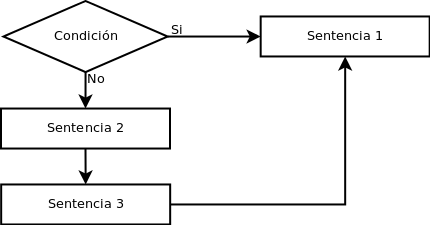
\includegraphics[width=200pt]{./Imagenes/condicionsimple.png}
\end{center}

A continuación, un código de ejemplo. La primera linea indica que si (y solo si) se cumple la condición dada, se va a realizar la sentencia 1. La tercera linea indica que si no se cumple la condición se realiza la sentencia 2. El end que aparece en la cuarta linea se utiliza para finalizar la bifurcación.

\begin{lstlisting}[language=Matlab]
if condicion
    sentencia 1
else sentencia 2
end
\end{lstlisting}

\paragraph{Ejemplo 1}

Crear un programa en el que se introduzcan dos números por el teclado y que nos diga cual es el mayor.

\begin{lstlisting}[language=Matlab]
a = input('Ingrese un numero')
b = input('Ingrese otro numero')
if a > b
    disp ('El primer numero es mayor que el segundo')
else 
    disp ('El segundo numero es mayor que el primero')
end
\end{lstlisting}

\section{Condiciones múltiples}

La sntaxis es de la siguiente forma:\\
\begin{lstlisting}[language=Matlab]
if condicion 1
    sentencia 1
elseif condicion 2
    sentencia 2
elseif condicion 3
    sentencia 3
end
\end{lstlisting}

\paragraph{Ejemplo 1}

Crear un programa tal que un usuario introduzca un numero del 0-9 y un segundo usuario tenga que acertarlo.\\
\begin{lstlisting}[language=Matlab]
a = input('Ingrese un numero entre 0 y 9:')
if n>9 | n<0
    disp('Ingrese un numero correcto')
    return
end
clc
b = input('Intenta adivinar:')
if g==n
    disp('Correcto!')
else
    disp('Incorrecto')
end
\end{lstlisting}

\paragraph{Ejemplo 2}

Crear un programa tal que un usuario introduzca un numero por teclado, que diga si es entero y luego si es par o impar.\\
\begin{lstlisting}[language=Matlab]
a = input('Ingrese un numero:')
y = abs(a)
if a==y
    disp('El numero es entero')
    entero = abs(a)
    if entero == a
        disp('Es par')
    else
        disp('Es impar')
    end
else
    disp('El numero no es entero')
end
\end{lstlisting}

\begin{lstlisting}[language=Matlab]

\end{lstlisting}


\section{Códigos de ejemplo}

\subsection{Manipulación de matrices}

\begin{lstlisting}[language=Matlab]
% Ejercicio 3. Manipulacion de matrices

format compact
echo on

% A) Almacena en memoria principal la siguiente matriz, en una variable que
% se llame M1:
M1 = [1 2 3; -3 -4 4; 3 7 2]

% B) Calcula la traspuesta de M1 y guardala en M2
M2 = M1'

% C) Calcula el producto elemento a elemento de M1 y M2
M1.*M2

% D) Calcula la suma de M1 y M2
M1+M2

% E) Calcula la division elemento a elemento de M1 y M2
M1./M2

% F) Calcula el producto matricial de M1 y M2 y guardalo en prodM1M2
prodM1M2 = M1 * M2

% G) Calcula el producto matricial de M2 y M1 y guardalo en prodM2M1
prodM2M1 = M2 * M1
% H) Calcula la division matricial de M1 y M2
M1/M2

% I) Cambia el valor del elemento central de M1 a 9
M1(2,2) = 9

% J) Guarda en una matriz llamada esquinasM1 de tamano 2x2 los elementos de
% las esquinas de M1
esquinasM1 = M1([1 end], [1 end])

% K) Guarda en un vector fila v los elementos de la diagonal principal de
% M1
v = [M1(1,1) M1(2,2) M1(3,3)]

% L) Guarda en un vector columna w los elementos de la diagonal secundaria
% de M2
w = [M2(1,3) M2(2,2) M2(3,1)]

% M) Calcula el producto escalar de v y w
v*w'
dot(v,w)

% N) Calcula el producto vectorial de v y w
[v(2)*w(3)-v(3)*w(2) v(3)*w(1)-v(1)*w(3) v(1)*w(2)-v(2)*w(1)]
cross(v,w)

% O) Guarda en fila1 los elementos de la primera fila de la matriz M1
fila1 = M1(1,:)

% P) Guarda en columna1 los elementos de la primera columna de la matriz M1
columna1 = M1(:,1)

% Q) convierte fila1 en un vector columna y columna1 e un vector fila.
fila1 = fila1'
columna1 = columna1'

% R) Genera un vector llamado angulos que tenga los angulos mutiplos de 30
% entre 30 y 360
angulos = 30:30:360

% S) Anade el elemento 0 en la primera posicion a angulos
angulos = [0 angulos]

% T) Extrae de ese vector los elementos con indice par (es decir, el
% segundo, el cuarto, el sexto, etc) y guardalos en angulosPar
angulosPar = angulos(2:2:end)

% U) Extrae de ese vector los elementos con indice impar (es decir, el
% primero, el tercero, el quinto, etc) y guardalos en angulosImpar
angulosImpar = angulos(1:2:end)

% V) Concatena a angulosPar el vector angulosImpar
angulosPar = [angulosPar angulosImpar]

echo off
format loose
\end{lstlisting}




\subsection{Matrices multidimensionales}
\begin{lstlisting}[language=Matlab]
% Ejercicio 4. Matrices multidimensionales

format compact
echo on

% En una urbanizacion hay 4 bloques de pisos, de 6 plantas cada uno. En
% cada una de las plantas hay 5 pisos, con un numero diferentes de
% habitaciones cada uno. Todas las puertas numero 1 y 2 son pisos de dos
% habitaciones, las puertas 3 y 4 son pisos de tres habitaciones y las
% puertas 5, tiene cuatro habitaciones. Se pide:

% Necesitamos crear una matriz que contendra el numero de habitaciones de
% cada apartamento. Como hay que distinguir entre bloque (1 a 4), planta (1
% a 6) y puerta (1 a 5), necesitaremos tres dimensiones.
plantas = 6
puertas = 5
bloques = 4
urb = zeros(plantas, puertas, bloques);
urb(:, [1 2], :) = 2;       % Todas las puertas 1 y 2 tienen 2 habitaciones
urb(:, [3 4], :) = 3;       % Todas las puertas 3 y 4 tienen 3 habitaciones
urb(:, 5, :) = 4            % Todas las puertas 5     tienen 4 habitaciones

% Imprimir bloque por bloque el numero de habitaciones de cada piso.
urb(:,:,1)
urb(:,:,2)
urb(:,:,3)
urb(:,:,4)

% Imprimir el numero de habitaciones de todos los pisos de la planta 4 del
% bloque 2.
urb(4, :, 2)

% Imprimir el numero de habitaciones del piso 3 de la planta 2 del bloque
% 3.
urb(2, 3, 3)

% Calcular e imprimir el numero total de habitaciones de cada bloque.
sum(sum(urb))

% Calcular e imprimir el numero total de habitaciones de la urbanizacion.
sum(sum(sum(urb)))

echo off
format loose
\end{lstlisting}



\subsection{Distancia}
\begin{lstlisting}[language=Matlab]
% Ejercicio 5. Distancia

format compact
echo on

% Define dos vectores de tres elementos (x, y, z), que representan las
% coordenadas 3D de dos puntos en el espacio.
a = [1 3 5]
b = [4 1 0]

% Calcula la distancia que hay entre ambos puntos.
d = sqrt(sum((a-b).^2))

echo off
format loose
\end{lstlisting}


\subsection{Vectores}

\begin{lstlisting}[language=Matlab]
% Ejercicio 6. Diferencias

format compact
echo on

% Crea el vector V con los valores 3, 4, 9, 5, 2, 1, 5, 3, 9, 8, 4, 6, 2, 1, 6, 5.
V = [3 4 9 5 2 1 5 3 9 8 4 6 2 1 6 5]

% Calcula un nuevo vector D con las diferencias entre los elementos
% consecutivos, de forma que Di=V(i+1)?V(i)
% El resultado ha de ser 1, 5, -4, -3, -1, 4, -2, 6, -1, -4, 2, -4, -1, 5, -1.
D = V(2:end)-V(1:end-1)

echo off
format loose
\end{lstlisting}



\subsection{Operaciones en Matlab}
\begin{lstlisting}[language=Matlab]
% Ejercicio 7. Operaciones en Matlab

format compact
echo on

% Apartado A

% Sean los vectores a=[2 4 3 3] y b=[5 2 3 4].
a=[2 4 3 3]
b=[5 2 3 4]

% Calcula todas las relaciones entre sus elementos (igualdad, mayor o
% igual, mayor...)
a==b
a>b
a<b
a>=b
a<=b
a~=b

% Apartado B

% Con dos de los vectores cualesquiera que te dieron como resultado alguna
% de las operaciones anteriores, aplica los operadores AND, OR y NOT.
a>=b & a<=b
a>b | a<b
~(a==b)

% Apartado C

% Genera un vector entre 0 y 2*pi con un salto de pi/8. Calcula e imprime
% todas las magnitudes trigonometricas disponibles en Matlab.
g = 0:pi/8:2*pi
sin(g)
cos(g)
tan(g)

% Apartado D
% Calcula el maximo y la posicion que ocupa dicho elemento del vector b del
% apartado A.
b
[maximo posicion] = max(b)

% Apartado E

% Sea x=5.678.
x=5.678

% Calcula todos los posibles redondeos de x disponibles en Matlab.
round(x)    % redondeo hacia el entero mas proximo
fix(x)      % redondea hacia el entero mas proximo a 0
floor(x)    % valor entero mas proximo hacia -infinito
ceil(x)     % valor entero mas proximo hacia +infinito

% Apartado F

% Sea el vector c=[5 3 2 7 4 11 25 -4 1]
c=[5 3 2 7 4 11 25 -4 1]

% Calcula el menor y el mayor de los elementos del vector.
minc = min(c)
maxc = max(c)

% Guarda en COrden el vector ordenado de c.
COrden = sort(c)

% Apartado G

% Genera una matriz de ceros de tamano 50x50.
m = zeros(50,50)

% Coloca unos en las posiciones (3,4), (32,25) y (49,49).
m(3,4) = 1;
m(32,25) = 1;
m(49,49) = 1

% Busca a continuacion en esta matriz todos los elementos distintos de cero.
find(m)

% Convierte esta matriz en una matriz dispersa.
m = sparse(m)

% Apartado H

% Almacena en memoria principal la siguiente matriz, en una variable que se
% llame M1
M1 = [1 2 3; -3 -4 4; 3 7 2]

% Apartado I

% Calcua el determinante de la matriz y calcula la matriz inversa
% guardandola en M1inv.
det(M1)
M1inv = M1^-1

% Apartado J

% A continuacion, guarda en el fichero result.txt la matriz M1inv en
% formato ascii.
save 'M1inv.dat' M1inv -ascii

% Apartado K

% Lee este fichero y guarda el contenido en la matriz M1inv2.
load 'M1inv.dat' M1inv2 -ascii

% Apartado L

% Haz diferentes pruebas de lectura y escritura de matrices en ficheros
% binarios.
save M1inv M1inv
clear M1inv
load 'M1inv.mat'
% etc...

echo off
format loose
\end{lstlisting}


\subsection{Tabla de conversión de temperaturas}
\begin{lstlisting}[language=Matlab]
% Ejercicio 8. Tabla de conversion de temperaturas

format compact
echo on

% Construye una tabla de cuatro columnas. La primera contendra temperaturas
% Celsius desde 0 hasta 100, de medio en medio grado, a segunda contendra
% la temperatura Fahrenheit, la siguiente sera Kelvin y, por ultimo, Reamur.

% Temperaturas en C
C = 0:0.5:100

% Temperaturas en F
F = 9/5 * C + 32

% Temperaturas en K
K = C + 273.15

% Temperaturas en R
R = 8/10 * C

% Composicion en forma de tabla de cuatro columnas
Tabla = [C' F' K' R']

echo off
format loose
\end{lstlisting}


\subsection{Ecuación de una recta en el plano}
\begin{lstlisting}[language=Matlab]
% Ejercicio 9. Ecuacion de una recta en el plano

format compact
echo on

% Escribe dos vectores que representan dos puntos en el plano
v1 = [10 3]
v2 = [7 -2]

% Calcula el vector de coeficientes (a, b, c) de la ecuacion general de la
% recta que los une.
coef = [v2(2)-v1(2)  v1(1)-v2(1)  v1(2)*v1(2)-v2(2)*v1(1)]

echo off
format loose
\end{lstlisting}


\subsection{Sumatoria}
\begin{lstlisting}[language=Matlab]
% Ejercicio 10. Sumatoria

format compact
echo on

% Escribe una expresion que calcule la suma de todos los numeros naturales
% hasta n.

% Para este caso, sea n = 100
n = 100
sum(1:n)

% Los listillos, como Gauss, pensaran que al anterior metodo es demasiado
% burdo, asi que podemos usar el metodo que el propio Gauss empleo cuando
% su profesor quiso mantener a los alumnos entretenidos hadiendo sumas
% durante un buen rato:
(1+n)/2 * n

echo off
format loose
\end{lstlisting}


\subsection{Factorial}
\begin{lstlisting}[language=Matlab]
% Ejercicio 11. Factorial

format compact
echo on

% Escribe una expresion que calcule el factorial de n.

% Para este caso, sea n = 10
n = 10
prod(1:n)

% Matlab dispone de la funcion factorial, que podemos usar en este caso:
factorial(n)

echo off
format loose
\end{lstlisting}


\subsection{Detección de palíndromos}
\begin{lstlisting}[language=Matlab]
% Ejercicio 12. Deteccion de palindromos

format compact
echo on

% Utilizaremos la siguiente secuencia de caracteres
sec='dabalearrozalazorraelabad'

% Podemos comparar la cadena con la misma cadena invertida
% La cadena invertida es:
inv = sec(length(sec):-1:1)

% Comprobamos si la cadena es igual a la cadena invertida
all(sec==inv)

echo off
format loose
\end{lstlisting}


\subsection{DNI}
\begin{lstlisting}[language=Matlab]
% Ejercicio 13. DNI

format compact
echo on

% Almacenamos las letras en una cadena para seleccionarlas con facilidad
letras = 'TRWAGMYFPDXBNJZSQVHLCKE';

% Determinamos el numero de DNI del que vamos a calcular la letra de
% control
DNI = 12345678;

% Calculamos la letra
% El resto de la division por 23 se calcula mendiante la funcion MOD
% Este resto toma valores de 0 a 22, mientras que las posiciones de las
% letras en la cadena van de 1 a 23. Por ello, sumamos 1 al resto obtenido.
letra = letras(mod(DNI, 23)+1)

echo off
format loose
\end{lstlisting}


\subsection{Área y perímetro de polígonos}
\begin{lstlisting}[language=Matlab]
% Ejercicio 14. area y Perimetro de poligonos

format compact
echo on

% Definimos las coordenadas de los vertices de un poligono arbitrario
% El primer y ultimo vertice tienen el mismo valor para simplificar el
% calculo
x=[0 1 2 1 0];
y=[0 0 1 1 0];

% Definimos cuatro variables auxiliares para evitar su calculo reptidas
% veces
x1 = x(1:end-1);    % Todos los valores de x excepto el ultimo
x2 = x(2:end);      % todos los valores de x excepto el primero
y1 = y(1:end-1);    % Todos los valores de y excepto el ultimo
y2 = y(2:end);      % todos los valores de y excepto el primero

% Calculo del perimetro:
% La matriz de distancias en x entre cada par de puntos consecutivos viene
% dada por x1-x2
% La matriz de distancias en y entre cada par de puntos consecutivos viene
% dada por y1-y2
% La matriz de distancias entre cada par de puntos consecutivos viene dada
% por sqrt((x1-x2).^2 + (y1-y2).^2)
% El perimetro es la suma de dichas distancias
perim = sum(sqrt((x1-x2).^2 + (y1-y2).^2))

% Calculo del area:
% Aplicando la formula del enunciado se obtiene:
area = sum(x1.*y2 - x2.*y1) / 2

% No obstante, esa expresion es equivalente a
% (sum(x1.*y2) - sum(x2.*y1)) / 2
% y cada uno de los anteriores sumatorios se trata en realidad de un
% producto escalar. Tal como vimos en un ejercicio anterior, el producto
% escalar de dos vectores se puede calcular mediante el producto matricial
% de un vector fila por un vector columna.
% La expresion, por lo tanto, queda asi:
area = (x1*y2' - x2*y1') / 2

echo off
format loose
\end{lstlisting}


\subsection{Chargaff}
\begin{lstlisting}[language=Matlab]
% Ejercicio 15. Chargaff

echo on
format compact

% Utilizamos la siguiente secuencia de ADN como ejemplo
adn = 'AGCTGGTACCTGACCGGTACGATTGAC';

% Contamos la cantidad de cada una de las bases
nA = sum(adn=='A')
nT = sum(adn=='T')
nG = sum(adn=='G')
nC = sum(adn=='C')

% Calculamos los coeficientes de Chargaff
a = (nA-nT)/(nA+nT)
c = (nC-nG)/(nC+nG)


echo off
format loose
\end{lstlisting}




\subsection{Derivación de polinomios}
\begin{lstlisting}[language=Matlab]
% Ejercicio 16. Derivacion de polinomios

format compact
echo on

% Definimos un polinomio mediante un vector que contiene sus coeficientes
% ordendos de mayor a menor grado
pol = [3 4 1 -2 5 -1 4 2]

% Creamos una variable auxiliar que contiene los grados de mayor a menor
% hasta uno
gra = length(pol)-1:-1:1

% Calculamos la derivada
der = pol(1:end-1) .* gra

echo off
format loose
\end{lstlisting}



\subsection{Solución de sistemas de ecuaciones lineales}
\begin{lstlisting}[language=Matlab]
% Ejercicio 17. Solucion de sistemas de ecuaciones lineales

format compact
echo on

% Un sistema de ecuaciones lineales puede representarse mediante una
% expresion matricial AX=B
% Multiplicando la inversa de A por la izquierda resulta X = A^-1 x B, por
% lo que es posible relolver sistemas de ecuaciones lineales mediante la ultima expresion.
% Define la matriz A y el vector B que representan el sistema lineal
A = [1 -2 4 3; 2 5 -2 3; 5 8 0 -3; 4 0 -1 5]
B = [1; -2; 3; 0]

% Calcula la solucion X.
X = A^-1 * B

echo off
format loose
\end{lstlisting}



\subsection{Los mercados}
\begin{lstlisting}[language=Matlab]
% Ejercicio 18. La bolsa

format compact
echo on

% Disponemos de un vector de numeros que representan el valor
% del IBEX35 al cierre de cada sesion diaria, durante una cierta
% cantidad de dias. IBEX35 = [1345 1326 1261 ...]
% El primer elemento corresponde al dia 1, el segundo al dia 2,
% y asi sucesivamente.

ibex = [11693 11903 11849 11180 11139 11554 11350 11180 ...
        11136 11412 10799 10911 10661 10631 11557 11328 ...
        11176 11112 11438 11387 10945 10987]

% Nos interesa calcular:
% 1. Cual es el maximo incremento producido entre un dia y el siguiente
% 2. Que dia se ha producido dicho incremento
% 3. Que dias se ha producido un descenso
% 4. Que dias se ha producido un descenso superior al 5%
% 5. Que dias se han producido maximos (valor mayor que el dia anterior

% 1. Cual es el maximo incremento producido entre un dia y el siguiente

% Supongamos que la variable que contiene los valores se llama ibex.
% El valor del IBEX 35 en todos los dias menos el primero es
ibex(2:end)

% Y el valor en los dias primero a penultimo
ibex(1:end-1)

% El vector de diferencias entre cada dia y el anterior es la diferencia
% entre ambos vectores. Podemos crear la variable var para guardar dicho
% vector de diferencias, y que las sucesivas expresiones queden mas claras:
var = ibex(2:end) - ibex(1:end-1)

% La anterior expresion nos da la variacion de cada dia con respecto al
% anterior. Obviamente, no tenemos el dato para el primer dia.
% Como queremos saber el maximo incremento, utilizamos la funcion max:
max(var)

% Solucion:
var = ibex(2:end) - ibex(1:end-1)
max(var)

% 2. Que dia se ha producido dicho incremento

% Se trata de buscar el maximo recien hallado dentro del vector de
% variaciones diarias. Podemos comparar el vector de variaciones con
% el valor (escalar) del maximo ya encontrado:
var == max(var)

% Asi obtenemos un vector de valores logicos, con 1 (verdadero) en
% aquellas posiciones en las que se produce la coincidencia. Para conocer
% la posicion de la(s) coincidencia(s) usaremos la funcion find:
find(var == max(var))

% Pero como la primera posicion de var corresponde al dia 2, tenemos que
% sumar 1 a la posicion encontrada para que el resultado sea el dia correcto.

% Solucion:
find(var == max(var)) + 1

% 3. Que dias se ha producido un descenso

% La condicion de descenso es
var < 0

% Esa expresion genera un vector logico con unos en las posiciones
% donde var es menor que 0. Siguiendo el mismo razonamiento del anterior
% apartado, encontramos los dias mediante la funcion find y sumando 1.

% Solucion:
find(var < 0) + 1

% 4. Que dias se ha producido un descenso superior al 5%

% La variacion relativa (tanto por 1) se calcula dividiendo la variacion
% habida entre cada dos dias entre el valor absoluto:
rel = var ./ ibex(1:end-1)

% Queremos encontrar en que dias la variacion relativa es menor que -0,05
% (descenso superior al 5%):
find(rel < -0.05)

% Y le anadimos 1 para referirnos a los dias correctos.

% Solucion:
rel = var ./ibex(1:end-1)
find(rel < -0.05) + 1

% 5. Que dias se han producido maximos (valor mayor que el dia anterior
% y que el siguiente)

% Este calculo solo se puede hacer sobre los valores 2 a penultimo,
% es decir, sobre
ibex(2:end-1)

% La condicion de que uno de esos dias tenga un valor mayor que el anterior es
ibex(2:end-1) > ibex(1:end-2)

% y la condicion de que un dia tenga un valor mayor que el siguiente es
ibex(2:end-1) > ibex(3:end)

% Las dos condiciones simultaneamente:
ibex(2:end-1) > ibex(1:end-2) & ibex(2:end-1) > ibex(3:end)

% Lo mismo que en otros apartados, el vector resultante comienza en el
% segundo dia, luego sumamos 1 al resultado para obtener el numero de dia correcto.

% Solucion:
find(ibex(2:end-1) > ibex(1:end-2) & ibex(2:end-1) > ibex(3:end)) + 1

echo off
format loose
\end{lstlisting}



\section{Legibilidad}

Frecuentemente el usuario de MATLAB escribe archivo M que le resultan de utilidad. Pasado un tiempo sin usar un archivo es posible que uno olvide que tarea realiza exactamente. En tal caso es necesario mirar el contenido del archivo y repasar su contenido. Es en este punto cuando se agradece (o se echa en falta) una buena practica de programación que haga que el código sea legible.\\

Los siguientes consejos ayudar sin duda al usuario de MATLAB a conseguir programas legibles.
\begin{itemize}
\item Elegir nombres de variables indicativos de lo que representan.
\item No usar una misma variable para representar mas que una cosa.
\item Incluir comentarios en el código para ayudar a seguir la secuencia del programa.
\item Dividir el código en trozos, de forma tal que sea posible abarcar cada trozo de un vistazo en una ventana mediana. La división no ha de ser arbitraria, sino que los trozos deben tener cada uno cometidos claros. Normalmente los diagramas de flujo desarrollados con anterioridad a la codificación indican como realizar esta división.
\end{itemize}